% Options for packages loaded elsewhere
\PassOptionsToPackage{unicode}{hyperref}
\PassOptionsToPackage{hyphens}{url}
%
\documentclass[
]{article}
\title{Categorical variables with forcats 😼}
\usepackage{etoolbox}
\makeatletter
\providecommand{\subtitle}[1]{% add subtitle to \maketitle
  \apptocmd{\@title}{\par {\large #1 \par}}{}{}
}
\makeatother
\subtitle{Workshop: I2DS Tools for Data Science - Presentation
(tutorial)}
\author{Carolina Díaz \& Priscila Pimentel}
\date{November 2022}

\usepackage{amsmath,amssymb}
\usepackage{lmodern}
\usepackage{iftex}
\ifPDFTeX
  \usepackage[T1]{fontenc}
  \usepackage[utf8]{inputenc}
  \usepackage{textcomp} % provide euro and other symbols
\else % if luatex or xetex
  \usepackage{unicode-math}
  \defaultfontfeatures{Scale=MatchLowercase}
  \defaultfontfeatures[\rmfamily]{Ligatures=TeX,Scale=1}
\fi
% Use upquote if available, for straight quotes in verbatim environments
\IfFileExists{upquote.sty}{\usepackage{upquote}}{}
\IfFileExists{microtype.sty}{% use microtype if available
  \usepackage[]{microtype}
  \UseMicrotypeSet[protrusion]{basicmath} % disable protrusion for tt fonts
}{}
\makeatletter
\@ifundefined{KOMAClassName}{% if non-KOMA class
  \IfFileExists{parskip.sty}{%
    \usepackage{parskip}
  }{% else
    \setlength{\parindent}{0pt}
    \setlength{\parskip}{6pt plus 2pt minus 1pt}}
}{% if KOMA class
  \KOMAoptions{parskip=half}}
\makeatother
\usepackage{xcolor}
\IfFileExists{xurl.sty}{\usepackage{xurl}}{} % add URL line breaks if available
\IfFileExists{bookmark.sty}{\usepackage{bookmark}}{\usepackage{hyperref}}
\hypersetup{
  pdftitle={Categorical variables with forcats 😼},
  pdfauthor={Carolina Díaz \& Priscila Pimentel},
  hidelinks,
  pdfcreator={LaTeX via pandoc}}
\urlstyle{same} % disable monospaced font for URLs
\usepackage[margin=1in]{geometry}
\usepackage{color}
\usepackage{fancyvrb}
\newcommand{\VerbBar}{|}
\newcommand{\VERB}{\Verb[commandchars=\\\{\}]}
\DefineVerbatimEnvironment{Highlighting}{Verbatim}{commandchars=\\\{\}}
% Add ',fontsize=\small' for more characters per line
\usepackage{framed}
\definecolor{shadecolor}{RGB}{248,248,248}
\newenvironment{Shaded}{\begin{snugshade}}{\end{snugshade}}
\newcommand{\AlertTok}[1]{\textcolor[rgb]{0.94,0.16,0.16}{#1}}
\newcommand{\AnnotationTok}[1]{\textcolor[rgb]{0.56,0.35,0.01}{\textbf{\textit{#1}}}}
\newcommand{\AttributeTok}[1]{\textcolor[rgb]{0.77,0.63,0.00}{#1}}
\newcommand{\BaseNTok}[1]{\textcolor[rgb]{0.00,0.00,0.81}{#1}}
\newcommand{\BuiltInTok}[1]{#1}
\newcommand{\CharTok}[1]{\textcolor[rgb]{0.31,0.60,0.02}{#1}}
\newcommand{\CommentTok}[1]{\textcolor[rgb]{0.56,0.35,0.01}{\textit{#1}}}
\newcommand{\CommentVarTok}[1]{\textcolor[rgb]{0.56,0.35,0.01}{\textbf{\textit{#1}}}}
\newcommand{\ConstantTok}[1]{\textcolor[rgb]{0.00,0.00,0.00}{#1}}
\newcommand{\ControlFlowTok}[1]{\textcolor[rgb]{0.13,0.29,0.53}{\textbf{#1}}}
\newcommand{\DataTypeTok}[1]{\textcolor[rgb]{0.13,0.29,0.53}{#1}}
\newcommand{\DecValTok}[1]{\textcolor[rgb]{0.00,0.00,0.81}{#1}}
\newcommand{\DocumentationTok}[1]{\textcolor[rgb]{0.56,0.35,0.01}{\textbf{\textit{#1}}}}
\newcommand{\ErrorTok}[1]{\textcolor[rgb]{0.64,0.00,0.00}{\textbf{#1}}}
\newcommand{\ExtensionTok}[1]{#1}
\newcommand{\FloatTok}[1]{\textcolor[rgb]{0.00,0.00,0.81}{#1}}
\newcommand{\FunctionTok}[1]{\textcolor[rgb]{0.00,0.00,0.00}{#1}}
\newcommand{\ImportTok}[1]{#1}
\newcommand{\InformationTok}[1]{\textcolor[rgb]{0.56,0.35,0.01}{\textbf{\textit{#1}}}}
\newcommand{\KeywordTok}[1]{\textcolor[rgb]{0.13,0.29,0.53}{\textbf{#1}}}
\newcommand{\NormalTok}[1]{#1}
\newcommand{\OperatorTok}[1]{\textcolor[rgb]{0.81,0.36,0.00}{\textbf{#1}}}
\newcommand{\OtherTok}[1]{\textcolor[rgb]{0.56,0.35,0.01}{#1}}
\newcommand{\PreprocessorTok}[1]{\textcolor[rgb]{0.56,0.35,0.01}{\textit{#1}}}
\newcommand{\RegionMarkerTok}[1]{#1}
\newcommand{\SpecialCharTok}[1]{\textcolor[rgb]{0.00,0.00,0.00}{#1}}
\newcommand{\SpecialStringTok}[1]{\textcolor[rgb]{0.31,0.60,0.02}{#1}}
\newcommand{\StringTok}[1]{\textcolor[rgb]{0.31,0.60,0.02}{#1}}
\newcommand{\VariableTok}[1]{\textcolor[rgb]{0.00,0.00,0.00}{#1}}
\newcommand{\VerbatimStringTok}[1]{\textcolor[rgb]{0.31,0.60,0.02}{#1}}
\newcommand{\WarningTok}[1]{\textcolor[rgb]{0.56,0.35,0.01}{\textbf{\textit{#1}}}}
\usepackage{graphicx}
\makeatletter
\def\maxwidth{\ifdim\Gin@nat@width>\linewidth\linewidth\else\Gin@nat@width\fi}
\def\maxheight{\ifdim\Gin@nat@height>\textheight\textheight\else\Gin@nat@height\fi}
\makeatother
% Scale images if necessary, so that they will not overflow the page
% margins by default, and it is still possible to overwrite the defaults
% using explicit options in \includegraphics[width, height, ...]{}
\setkeys{Gin}{width=\maxwidth,height=\maxheight,keepaspectratio}
% Set default figure placement to htbp
\makeatletter
\def\fps@figure{htbp}
\makeatother
\setlength{\emergencystretch}{3em} % prevent overfull lines
\providecommand{\tightlist}{%
  \setlength{\itemsep}{0pt}\setlength{\parskip}{0pt}}
\setcounter{secnumdepth}{-\maxdimen} % remove section numbering
\ifLuaTeX
  \usepackage{selnolig}  % disable illegal ligatures
\fi

\begin{document}
\maketitle

{
\setcounter{tocdepth}{2}
\tableofcontents
}
\begin{center}\rule{0.5\linewidth}{0.5pt}\end{center}

\hypertarget{outline}{%
\section{Outline}\label{outline}}

\begin{enumerate}
\def\labelenumi{\arabic{enumi}.}
\tightlist
\item
  Recall: Categorical data as factors
\item
  Functions:
\end{enumerate}

\begin{itemize}
\tightlist
\item
  \texttt{fct\_inorder()}
\item
  \texttt{fct\_infreq()}
\item
  \texttt{fct\_rev()}
\item
  \texttt{fct\_reorder()}
\item
  \texttt{fct\_relevel()}
\item
  \texttt{fct\_lump()}
\item
  \texttt{fct\_recode()}
\item
  \texttt{fct\_collapse()}
\end{itemize}

\begin{enumerate}
\def\labelenumi{\arabic{enumi}.}
\setcounter{enumi}{2}
\tightlist
\item
  Exercises
\end{enumerate}

\hypertarget{categorical-data-as-factors}{%
\section{Categorical data as
factors}\label{categorical-data-as-factors}}

Let's remember that 📖, unlike a numerical variable, a categorical one
has a limited measurement scale or possible values, i.e.~categories or
levels in R.

Categorical variables might take two types ✌️ of scales:

\begin{itemize}
\item
  Nominal: when the categories do not have an order: marital status,
  gender, religion affiliation, migrant status, blood type.
\item
  Ordinal: when the categories have an order: social class, risk rating,
  object condition (good, regular, bad).
\end{itemize}

Categorical variables are coded as factors in R 😮. Why 🙋? Among other
reasons, because factors are much easier to work with than characters 😅.

But treating this data as factors could lead to processing the data in
an inappropriate way 😧. As many of the functions automatically get
converted from characters to factors, then factors often are presented
in a non-helpful manner 😕.

Fortunately, tidyverse through \textbf{forcats} 😼 is here to provide
tools for dealing with categorical variables and to help us💪!

\begin{Shaded}
\begin{Highlighting}[]
\FunctionTok{library}\NormalTok{(dplyr)}
\FunctionTok{library}\NormalTok{(ggplot2)}
\FunctionTok{library}\NormalTok{(forcats)}
\FunctionTok{library}\NormalTok{(palmerpenguins)}
\FunctionTok{library}\NormalTok{(jsonlite)}
\end{Highlighting}
\end{Shaded}

\hypertarget{creating-factors}{%
\subsection{Creating factors}\label{creating-factors}}

Let's say we have a variable that records age status:

\begin{Shaded}
\begin{Highlighting}[]
\NormalTok{x1 }\OtherTok{\textless{}{-}} \FunctionTok{c}\NormalTok{(}\StringTok{"senior"}\NormalTok{, }\StringTok{"baby"}\NormalTok{, }\StringTok{"adult"}\NormalTok{)}
\end{Highlighting}
\end{Shaded}

If we record this variable as a string, it could not be display in a
useful way.

\begin{Shaded}
\begin{Highlighting}[]
\FunctionTok{sort}\NormalTok{(x1)}
\end{Highlighting}
\end{Shaded}

\begin{verbatim}
[1] "adult"  "baby"   "senior"
\end{verbatim}

To avoid this, we can create a factor, starting by listing all the valid
levels:

\begin{Shaded}
\begin{Highlighting}[]
\NormalTok{age\_levels }\OtherTok{\textless{}{-}} \FunctionTok{c}\NormalTok{(}\StringTok{"baby"}\NormalTok{, }\StringTok{"child"}\NormalTok{, }\StringTok{"teenager"}\NormalTok{, }\StringTok{"adult"}\NormalTok{, }\StringTok{"middle\_age"}\NormalTok{, }\StringTok{"senior"}\NormalTok{)}
\end{Highlighting}
\end{Shaded}

With the list of all valid levels, we can create a factor with the
\texttt{factor()}function:

\begin{Shaded}
\begin{Highlighting}[]
\NormalTok{y1 }\OtherTok{\textless{}{-}} \FunctionTok{factor}\NormalTok{(x1, }\AttributeTok{levels =}\NormalTok{ age\_levels)}
\NormalTok{y1}
\end{Highlighting}
\end{Shaded}

\begin{verbatim}
[1] senior baby   adult 
Levels: baby child teenager adult middle_age senior
\end{verbatim}

\begin{Shaded}
\begin{Highlighting}[]
\FunctionTok{sort}\NormalTok{(y1)}
\end{Highlighting}
\end{Shaded}

\begin{verbatim}
[1] baby   adult  senior
Levels: baby child teenager adult middle_age senior
\end{verbatim}

If we omit the levels, they will be taken from the data and displayed in
a alphabetical order:

\begin{Shaded}
\begin{Highlighting}[]
\FunctionTok{factor}\NormalTok{(x1)}
\end{Highlighting}
\end{Shaded}

\begin{verbatim}
[1] senior baby   adult 
Levels: adult baby senior
\end{verbatim}

\hypertarget{forcats-functions}{%
\section{Forcats functions}\label{forcats-functions}}

\hypertarget{ordering-the-levels}{%
\subsection{Ordering the levels}\label{ordering-the-levels}}

If it is our preference to keep the order of the levels of the first
appearance in the data, we can use the \texttt{fct\_inorder}function:

\begin{Shaded}
\begin{Highlighting}[]
\NormalTok{age }\OtherTok{\textless{}{-}}\NormalTok{ x1 }\SpecialCharTok{\%\textgreater{}\%} \FunctionTok{factor}\NormalTok{() }\SpecialCharTok{\%\textgreater{}\%} \FunctionTok{fct\_inorder}\NormalTok{()}
\NormalTok{age}
\end{Highlighting}
\end{Shaded}

\begin{verbatim}
[1] senior baby   adult 
Levels: senior baby adult
\end{verbatim}

\hypertarget{ordering-by-frequency}{%
\subsection{Ordering by frequency}\label{ordering-by-frequency}}

For better visualization, it is often useful to change the order of the
factor levels. Let's use the \emph{starwars} data set to explain. We can
plot a bar graph to visualize the most common hair color among the star
wars characters:

\begin{Shaded}
\begin{Highlighting}[]
\FunctionTok{ggplot}\NormalTok{(starwars, }\FunctionTok{aes}\NormalTok{(}\AttributeTok{x =}\NormalTok{ hair\_color)) }\SpecialCharTok{+} 
    \FunctionTok{geom\_bar}\NormalTok{() }\SpecialCharTok{+} 
    \FunctionTok{coord\_flip}\NormalTok{()  }
\end{Highlighting}
\end{Shaded}

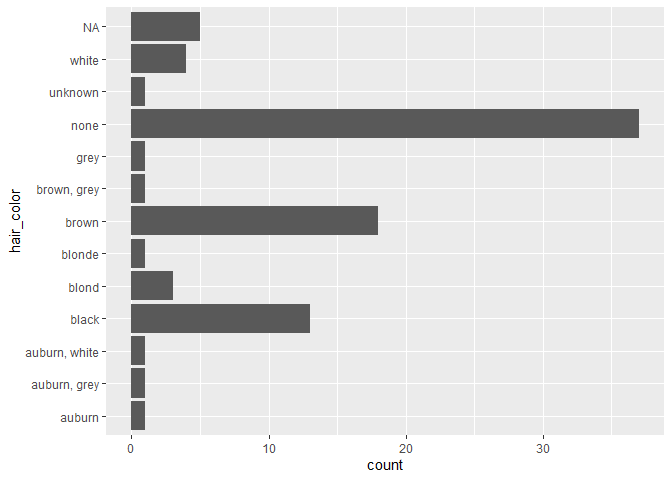
\includegraphics{Presentation_files/figure-latex/unnamed-chunk-9-1.pdf}

As we can see, this is a case of an unordered categorical variable. For
better visualization, we can reorder it by the frequency of haircolor.

For that, we can use the function \texttt{fct\_infreq()}:

\begin{Shaded}
\begin{Highlighting}[]
\FunctionTok{ggplot}\NormalTok{(starwars, }\FunctionTok{aes}\NormalTok{(}\AttributeTok{x =} \FunctionTok{fct\_infreq}\NormalTok{(hair\_color))) }\SpecialCharTok{+} 
  \FunctionTok{geom\_bar}\NormalTok{() }\SpecialCharTok{+} 
  \FunctionTok{coord\_flip}\NormalTok{()}
\end{Highlighting}
\end{Shaded}

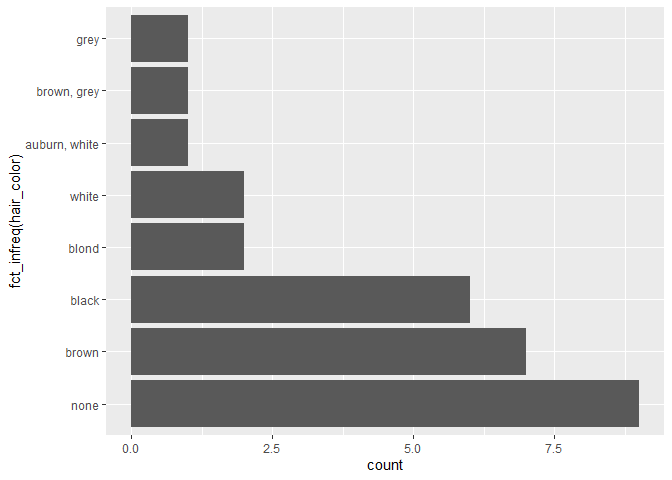
\includegraphics{Presentation_files/figure-latex/unnamed-chunk-10-1.pdf}

We can notice that NA by default is placed at the top. Also, we can see
that it is automatically ordered in a decreasing way.

\hypertarget{reversing}{%
\subsection{Reversing}\label{reversing}}

For an ascendant order, we should reverse the order that was
automatically displayed in a descendant one. It is done by using the
\texttt{fct\_rev()}function:

\begin{Shaded}
\begin{Highlighting}[]
\NormalTok{starwars }\SpecialCharTok{\%\textgreater{}\%}
  \FunctionTok{mutate}\NormalTok{(}\AttributeTok{hair\_color =}\NormalTok{ hair\_color }\SpecialCharTok{\%\textgreater{}\%} \FunctionTok{fct\_infreq}\NormalTok{() }\SpecialCharTok{\%\textgreater{}\%} \FunctionTok{fct\_rev}\NormalTok{()) }\SpecialCharTok{\%\textgreater{}\%}
  \FunctionTok{ggplot}\NormalTok{(}\FunctionTok{aes}\NormalTok{(}\AttributeTok{y =}\NormalTok{ hair\_color)) }\SpecialCharTok{+}
    \FunctionTok{geom\_bar}\NormalTok{()}
\end{Highlighting}
\end{Shaded}

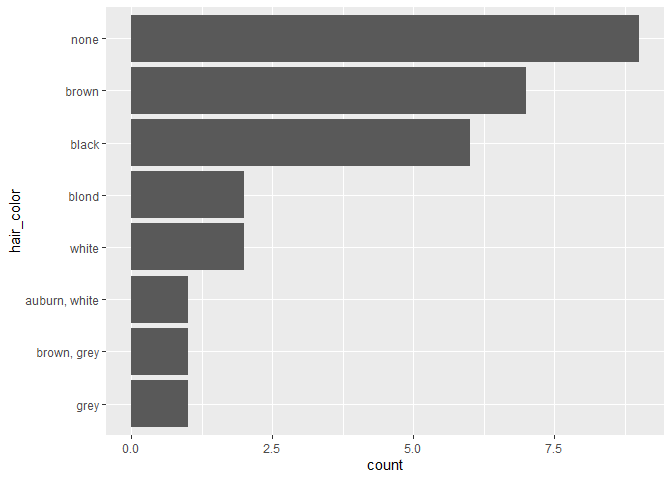
\includegraphics{Presentation_files/figure-latex/unnamed-chunk-11-1.pdf}

\hypertarget{ordering-by-another-variable}{%
\subsection{Ordering by another
variable}\label{ordering-by-another-variable}}

Let's take the \emph{gss\_cat} data set, from the \texttt{forcats}
package, to illustrate. Imagine we want to visualize how many hours in
average a person spends watching tv per day. We want to display this
statistic by the religion the person professes.

We can do that by plotting a geom\_point() graphic:

\begin{Shaded}
\begin{Highlighting}[]
\NormalTok{relig }\OtherTok{\textless{}{-}}\NormalTok{ gss\_cat }\SpecialCharTok{\%\textgreater{}\%}
  \FunctionTok{group\_by}\NormalTok{(relig) }\SpecialCharTok{\%\textgreater{}\%}
  \FunctionTok{summarise}\NormalTok{(}
    \AttributeTok{age =} \FunctionTok{mean}\NormalTok{(age, }\AttributeTok{na.rm =} \ConstantTok{TRUE}\NormalTok{),}
    \AttributeTok{tvhours =} \FunctionTok{mean}\NormalTok{(tvhours, }\AttributeTok{na.rm =} \ConstantTok{TRUE}\NormalTok{),}
    \AttributeTok{n =} \FunctionTok{n}\NormalTok{()}
\NormalTok{  )}

\FunctionTok{ggplot}\NormalTok{(relig, }\FunctionTok{aes}\NormalTok{(tvhours, relig)) }\SpecialCharTok{+} \FunctionTok{geom\_point}\NormalTok{()}
\end{Highlighting}
\end{Shaded}

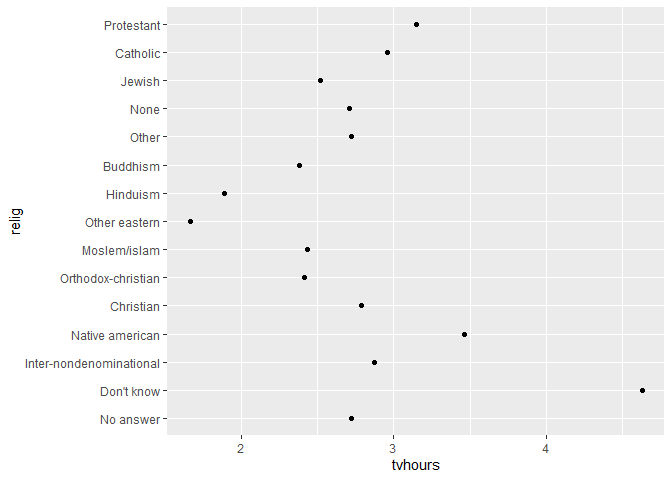
\includegraphics{Presentation_files/figure-latex/unnamed-chunk-12-1.pdf}

As we can see, the code gives back a disordered plot that makes it
harder to visualize and analyse information. Without an overall pattern,
it gets difficult to interpret the plot.

In this case, we want to order by religion. We can do this using the
\texttt{fct\_reorder()} function, which reorders one variable
(``relig'') by another (``tvhours'').

\begin{Shaded}
\begin{Highlighting}[]
\NormalTok{relig }\SpecialCharTok{\%\textgreater{}\%}
  \FunctionTok{mutate}\NormalTok{(}\AttributeTok{relig =} \FunctionTok{fct\_reorder}\NormalTok{(relig, tvhours)) }\SpecialCharTok{\%\textgreater{}\%}
  \FunctionTok{ggplot}\NormalTok{(}\FunctionTok{aes}\NormalTok{(tvhours, relig)) }\SpecialCharTok{+}
    \FunctionTok{geom\_point}\NormalTok{()}
\end{Highlighting}
\end{Shaded}

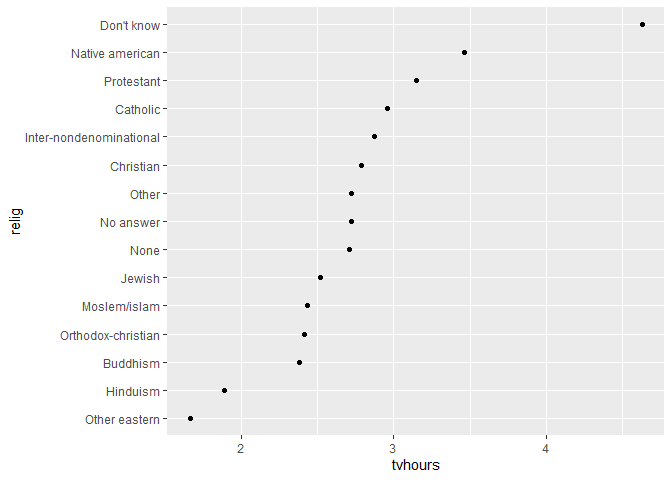
\includegraphics{Presentation_files/figure-latex/unnamed-chunk-13-1.pdf}

Now it is easy to point out which members of a certain religion watch
more/less tv and compare among these religions.

\hypertarget{manually-reordering}{%
\subsection{Manually reordering}\label{manually-reordering}}

Let's use now the \emph{palmerpenguins} dataset 🐧. This contains size
measurements for three penguin species observed on three islands in the
Palmer Archipelago, Antarctica. How is the distribution of the species?

\begin{Shaded}
\begin{Highlighting}[]
\NormalTok{penguins }\SpecialCharTok{\%\textgreater{}\%}
  \FunctionTok{count}\NormalTok{(species)}
\end{Highlighting}
\end{Shaded}

\begin{verbatim}
# A tibble: 3 x 2
  species       n
  <fct>     <int>
1 Adelie      152
2 Chinstrap    68
3 Gentoo      124
\end{verbatim}

\begin{Shaded}
\begin{Highlighting}[]
  \FunctionTok{ggplot}\NormalTok{(penguins,}\FunctionTok{aes}\NormalTok{(}\AttributeTok{y =}\NormalTok{ species)) }\SpecialCharTok{+}
  \FunctionTok{geom\_bar}\NormalTok{() }
\end{Highlighting}
\end{Shaded}

\includegraphics{Presentation_files/figure-latex/unnamed-chunk-14-1.pdf}

Notice that the species categories and the island are in alphabetical
order. This is the same order if you would plot it. If the data were
ordinal️, highly probable the categories would be ordered by the level
assigned to all possible categories, even with the ``non-answer'' in the
top 😰.

You may check the levels of the factor with the function
\texttt{levels()}, which prints them in order:

\begin{Shaded}
\begin{Highlighting}[]
\FunctionTok{levels}\NormalTok{(penguins}\SpecialCharTok{$}\NormalTok{species)}
\end{Highlighting}
\end{Shaded}

\begin{verbatim}
[1] "Adelie"    "Chinstrap" "Gentoo"   
\end{verbatim}

To tailor the data order as we need for our analytic purposes, we might
call the function \texttt{fct\_relevel()} to manually reorder the levels
of the factor. As second argument, you should make it explicit where you
want the categories.

\begin{Shaded}
\begin{Highlighting}[]
\NormalTok{penguins }\SpecialCharTok{\%\textgreater{}\%}
  \FunctionTok{mutate}\NormalTok{(}\AttributeTok{species =} \FunctionTok{fct\_relevel}\NormalTok{(species, }\StringTok{"Chinstrap"}\NormalTok{, }\StringTok{"Gentoo"}\NormalTok{, }\StringTok{"Adelie"}\NormalTok{)) }\SpecialCharTok{\%\textgreater{}\%}
  \FunctionTok{ggplot}\NormalTok{(}\FunctionTok{aes}\NormalTok{(}\AttributeTok{y =}\NormalTok{ species)) }\SpecialCharTok{+}
  \FunctionTok{geom\_bar}\NormalTok{()}
\end{Highlighting}
\end{Shaded}

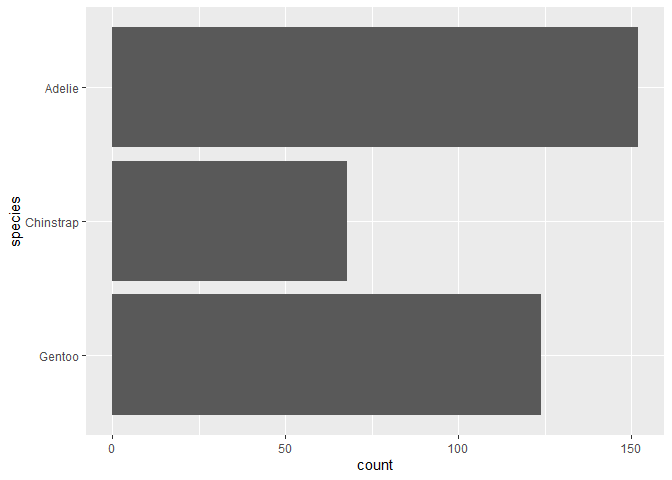
\includegraphics{Presentation_files/figure-latex/unnamed-chunk-16-1.pdf}

Even more, by default R moves the categories to the front, but if you
want to change this movement, you can point out that you want to place
the level after another with \texttt{after}.

\begin{Shaded}
\begin{Highlighting}[]
\FunctionTok{fct\_relevel}\NormalTok{(penguins}\SpecialCharTok{$}\NormalTok{species, }\FunctionTok{c}\NormalTok{(}\StringTok{"Adelie"}\NormalTok{), }\AttributeTok{after =} \DecValTok{1}\NormalTok{) }\SpecialCharTok{\%\textgreater{}\%}
  \FunctionTok{levels}\NormalTok{()}
\end{Highlighting}
\end{Shaded}

\begin{verbatim}
[1] "Chinstrap" "Adelie"    "Gentoo"   
\end{verbatim}

\begin{Shaded}
\begin{Highlighting}[]
\FunctionTok{fct\_relevel}\NormalTok{(penguins}\SpecialCharTok{$}\NormalTok{species, }\FunctionTok{c}\NormalTok{(}\StringTok{"Adelie"}\NormalTok{), }\AttributeTok{after =} \DecValTok{2}\NormalTok{) }\SpecialCharTok{\%\textgreater{}\%}
  \FunctionTok{levels}\NormalTok{()}
\end{Highlighting}
\end{Shaded}

\begin{verbatim}
[1] "Chinstrap" "Gentoo"    "Adelie"   
\end{verbatim}

Say you want to move the level to the end, then you indicate
\texttt{after} equal to \texttt{Inf}.

\begin{Shaded}
\begin{Highlighting}[]
 \FunctionTok{fct\_relevel}\NormalTok{(penguins}\SpecialCharTok{$}\NormalTok{species, }\FunctionTok{c}\NormalTok{(}\StringTok{"Chinstrap"}\NormalTok{), }\AttributeTok{after =} \ConstantTok{Inf}\NormalTok{) }\SpecialCharTok{\%\textgreater{}\%}
  \FunctionTok{levels}\NormalTok{()}
\end{Highlighting}
\end{Shaded}

\begin{verbatim}
[1] "Adelie"    "Gentoo"    "Chinstrap"
\end{verbatim}

\hypertarget{combining-levels}{%
\subsection{Combining levels}\label{combining-levels}}

Let's have a look at skin color of the star wars' characters:

\begin{Shaded}
\begin{Highlighting}[]
\NormalTok{starwars }\SpecialCharTok{\%\textgreater{}\%}
  \FunctionTok{count}\NormalTok{(skin\_color, }\AttributeTok{sort =} \ConstantTok{TRUE}\NormalTok{)}
\end{Highlighting}
\end{Shaded}

\begin{verbatim}
# A tibble: 31 x 2
   skin_color     n
   <chr>      <int>
 1 fair          17
 2 light         11
 3 dark           6
 4 green          6
 5 grey           6
 6 pale           5
 7 brown          4
 8 blue           2
 9 blue, grey     2
10 orange         2
# ... with 21 more rows
\end{verbatim}

Star wars characters have 31 skin colors. Who can
analyse/memorise/report the frequency of such a wide variety of skin
colors? Even if we were to graph this frequency, the graph would be very
long. So, let's simplify! Let's just choose the 5 most frequent skin
color of these characters and let's group the remaining in one category,
which we are going to call it as everybody else calls it: ``other''.

So, we might do this exploting the function \texttt{fct\_lump()} to
``lump'' all the least frequent skin colors. The number of levels to
keep is \texttt{n}.

\begin{Shaded}
\begin{Highlighting}[]
\NormalTok{starwars }\SpecialCharTok{\%\textgreater{}\%}
  \FunctionTok{mutate}\NormalTok{(}\AttributeTok{skin\_color =} \FunctionTok{fct\_lump}\NormalTok{(skin\_color, }\AttributeTok{n =} \DecValTok{5}\NormalTok{)) }\SpecialCharTok{\%\textgreater{}\%}
  \FunctionTok{count}\NormalTok{(skin\_color, }\AttributeTok{sort =} \ConstantTok{TRUE}\NormalTok{)}
\end{Highlighting}
\end{Shaded}

\begin{verbatim}
# A tibble: 6 x 2
  skin_color     n
  <fct>      <int>
1 Other         41
2 fair          17
3 light         11
4 dark           6
5 green          6
6 grey           6
\end{verbatim}

We can also use another grouping criterion. Let's use a frequency ratio:
let's only keep skin colours that have at least 10\% of the characters.
For this we will group using \texttt{prop}:

\begin{Shaded}
\begin{Highlighting}[]
\NormalTok{starwars }\SpecialCharTok{\%\textgreater{}\%}
  \FunctionTok{mutate}\NormalTok{(}\AttributeTok{skin\_color =} \FunctionTok{fct\_lump}\NormalTok{(skin\_color, }\AttributeTok{prop =}\NormalTok{ .}\DecValTok{1}\NormalTok{)) }\SpecialCharTok{\%\textgreater{}\%}
  \FunctionTok{count}\NormalTok{(skin\_color, }\AttributeTok{sort =} \ConstantTok{TRUE}\NormalTok{)}
\end{Highlighting}
\end{Shaded}

\begin{verbatim}
# A tibble: 3 x 2
  skin_color     n
  <fct>      <int>
1 Other         59
2 fair          17
3 light         11
\end{verbatim}

Only light and fair skin colour met the criterion of a frequency greater
than 10\%, so the remainder was grouped under ``other''.

Do you want to rename ``extra'' instead of ``other''? No problem: the
argument \texttt{other\_level} changes it:

\begin{Shaded}
\begin{Highlighting}[]
\NormalTok{starwars }\SpecialCharTok{\%\textgreater{}\%}
  \FunctionTok{mutate}\NormalTok{(}\AttributeTok{skin\_color =} \FunctionTok{fct\_lump}\NormalTok{(skin\_color, }\AttributeTok{prop =}\NormalTok{ .}\DecValTok{1}\NormalTok{, }\AttributeTok{other\_level =} \StringTok{"extra"}\NormalTok{)) }\SpecialCharTok{\%\textgreater{}\%}
  \FunctionTok{count}\NormalTok{(skin\_color, }\AttributeTok{sort =} \ConstantTok{TRUE}\NormalTok{)}
\end{Highlighting}
\end{Shaded}

\begin{verbatim}
# A tibble: 3 x 2
  skin_color     n
  <fct>      <int>
1 extra         59
2 fair          17
3 light         11
\end{verbatim}

Let's do something with a continuous variable of this base: height. Now,
we want to group it by the most frequent skin categories. Let's ask what
is the average height of the characters by skin colour? Let's just check
the 5 most popular skin colours and eliminate the \texttt{NA}.

\begin{Shaded}
\begin{Highlighting}[]
\NormalTok{avg\_height\_by\_skin\_color }\OtherTok{\textless{}{-}}\NormalTok{ starwars }\SpecialCharTok{\%\textgreater{}\%}
  \FunctionTok{mutate}\NormalTok{(}\AttributeTok{skin\_color =} \FunctionTok{fct\_lump}\NormalTok{(skin\_color, }\AttributeTok{n =} \DecValTok{5}\NormalTok{)) }\SpecialCharTok{\%\textgreater{}\%}
  \FunctionTok{group\_by}\NormalTok{(skin\_color) }\SpecialCharTok{\%\textgreater{}\%}
  \FunctionTok{summarise}\NormalTok{(}\AttributeTok{mean\_height =} \FunctionTok{mean}\NormalTok{(height, }\AttributeTok{na.rm =} \ConstantTok{TRUE}\NormalTok{))}
\NormalTok{avg\_height\_by\_skin\_color}
\end{Highlighting}
\end{Shaded}

\begin{verbatim}
# A tibble: 6 x 2
  skin_color mean_height
  <fct>            <dbl>
1 dark              183.
2 fair              177.
3 green             169 
4 grey              204.
5 light             170.
6 Other             169.
\end{verbatim}

\hypertarget{modifying-factor-levels}{%
\subsection{Modifying factor levels}\label{modifying-factor-levels}}

The forcats package is not only used to change the order of the levels
at our will. It is also used to change the order assigned of the levels
in the R code, i.e.~to recode the levels of the categories. To do this
we need the function \texttt{fct\_recode()}. This makes less temporary
but more permanent changes to the R code because it adjusts the labels
for publication and collapses the levels for making easy our analysis.

Let's look at the political spectrum of the \emph{gss\_cat} survey:

\begin{Shaded}
\begin{Highlighting}[]
\NormalTok{gss\_cat }\SpecialCharTok{\%\textgreater{}\%} \FunctionTok{count}\NormalTok{(partyid)}
\end{Highlighting}
\end{Shaded}

\begin{verbatim}
# A tibble: 10 x 2
   partyid                n
   <fct>              <int>
 1 No answer            154
 2 Don't know             1
 3 Other party          393
 4 Strong republican   2314
 5 Not str republican  3032
 6 Ind,near rep        1791
 7 Independent         4119
 8 Ind,near dem        2499
 9 Not str democrat    3690
10 Strong democrat     3490
\end{verbatim}

Labels are meaningless, aren't they? They are inconsistent. Let's make
our analysis more understandable: Let's tweak the labels, no matter if
they are longer, but better presented.

\begin{Shaded}
\begin{Highlighting}[]
\NormalTok{gss\_cat }\SpecialCharTok{\%\textgreater{}\%}
  \FunctionTok{mutate}\NormalTok{(}\AttributeTok{partyid =} \FunctionTok{fct\_recode}\NormalTok{(partyid,}
    \StringTok{"Republican, strong"}    \OtherTok{=} \StringTok{"Strong republican"}\NormalTok{,}
    \StringTok{"Republican, weak"}      \OtherTok{=} \StringTok{"Not str republican"}\NormalTok{,}
    \StringTok{"Independent, near rep"} \OtherTok{=} \StringTok{"Ind,near rep"}\NormalTok{,}
    \StringTok{"Independent, near dem"} \OtherTok{=} \StringTok{"Ind,near dem"}\NormalTok{,}
    \StringTok{"Democrat, weak"}        \OtherTok{=} \StringTok{"Not str democrat"}\NormalTok{,}
    \StringTok{"Democrat, strong"}      \OtherTok{=} \StringTok{"Strong democrat"}
\NormalTok{  )) }\SpecialCharTok{\%\textgreater{}\%}
  \FunctionTok{count}\NormalTok{(partyid)}
\end{Highlighting}
\end{Shaded}

\begin{verbatim}
# A tibble: 10 x 2
   partyid                   n
   <fct>                 <int>
 1 No answer               154
 2 Don't know                1
 3 Other party             393
 4 Republican, strong     2314
 5 Republican, weak       3032
 6 Independent, near rep  1791
 7 Independent            4119
 8 Independent, near dem  2499
 9 Democrat, weak         3690
10 Democrat, strong       3490
\end{verbatim}

We can even combine categories into a single new category if this makes
sense to us with the function \texttt{fct\_collapse}:

\begin{Shaded}
\begin{Highlighting}[]
\NormalTok{gss\_cat }\SpecialCharTok{\%\textgreater{}\%}
  \FunctionTok{mutate}\NormalTok{(}\AttributeTok{partyid =} \FunctionTok{fct\_collapse}\NormalTok{(partyid,}
    \AttributeTok{other =} \FunctionTok{c}\NormalTok{(}\StringTok{"No answer"}\NormalTok{, }\StringTok{"Don\textquotesingle{}t know"}\NormalTok{, }\StringTok{"Other party"}\NormalTok{),}
    \AttributeTok{rep =} \FunctionTok{c}\NormalTok{(}\StringTok{"Strong republican"}\NormalTok{, }\StringTok{"Not str republican"}\NormalTok{),}
    \AttributeTok{ind =} \FunctionTok{c}\NormalTok{(}\StringTok{"Ind,near rep"}\NormalTok{, }\StringTok{"Independent"}\NormalTok{, }\StringTok{"Ind,near dem"}\NormalTok{),}
    \AttributeTok{dem =} \FunctionTok{c}\NormalTok{(}\StringTok{"Not str democrat"}\NormalTok{, }\StringTok{"Strong democrat"}\NormalTok{)}
\NormalTok{  )) }\SpecialCharTok{\%\textgreater{}\%}
  \FunctionTok{count}\NormalTok{(partyid)}
\end{Highlighting}
\end{Shaded}

\begin{verbatim}
# A tibble: 4 x 2
  partyid     n
  <fct>   <int>
1 other     548
2 rep      5346
3 ind      8409
4 dem      7180
\end{verbatim}

\hypertarget{wrapping-up}{%
\section{Wrapping up}\label{wrapping-up}}

We might sum up the functions as:

\begin{itemize}
\tightlist
\item
  \texttt{fct\_inorder()} : Organizing the order in which they first
  appear.
\item
  \texttt{fct\_infreq()} : Reordering a factor by the frequency of
  values.
\item
  \texttt{fct\_rev()} : Reversing any criteria of ordering.
\item
  \texttt{fct\_reorder()} : Reordering a factor by another variable.
\item
  \texttt{fct\_relevel()} : Changing the order of a factor by hand.
\item
  \texttt{fct\_lump()} : Grouping the least/most frequent values of a
  factor into ``other''.
\item
  \texttt{fct\_recode()} : Clarifying labels of levels.
\item
  \texttt{fct\_collapse()}: Collapsing a lot of old levels into a new
  variable.
\end{itemize}

\hypertarget{references}{%
\section{References}\label{references}}

Pandas. (2022, November 11). Categorical data. Retrieved from pandas:
\url{https://pandas.pydata.org/docs/user_guide/categorical.html}

R for Data Science. (2022, November 12). R for Data Science. Retrieved
from R for Data Science:
\url{https://r4ds.had.co.nz/factors.html\#factors}

ScienceDirect. (2022, November 12). Categorical Variable. Retrieved from
ScienceDirect:
\url{https://www.sciencedirect.com/topics/mathematics/categorical-variable}

Wilke, C. (2022, November 12). The Wilke Lab - The University of Texas
at Austin. Retrieved from Getting things into the right order:
\url{https://wilkelab.org/SDS375/slides/getting-things-in-order.html\#16}

\end{document}
